\chapter{Design and Methodology}
\label{chap:method}

% The method you want to use to address the problem.
% Explicitly state verifiable hypotheses.

% Describe conceptual framework:
%
% - Root causes of HyTrack (from proposal, section 3.1).
%
% - Architecture of your proposed capability-based cookie isolation:
%
%   - Policies and capability structure (fields, signatures, flags).
%
%   - Browser-side enforcement logic.
%
%   - App-side integration (sending and receiving capabilities).
%
%   - Policy transmission via the installer or provider.
%
% - Diagrams: system overview, data flow between app, browser, and server.
%
% - Explain why this approach fulfills HyTrack’s three goals (seamless integration, feature completeness, and shared state control).


% ----------------------------Methodology--------------------------

\begin{figure}[h!]
  \centering
  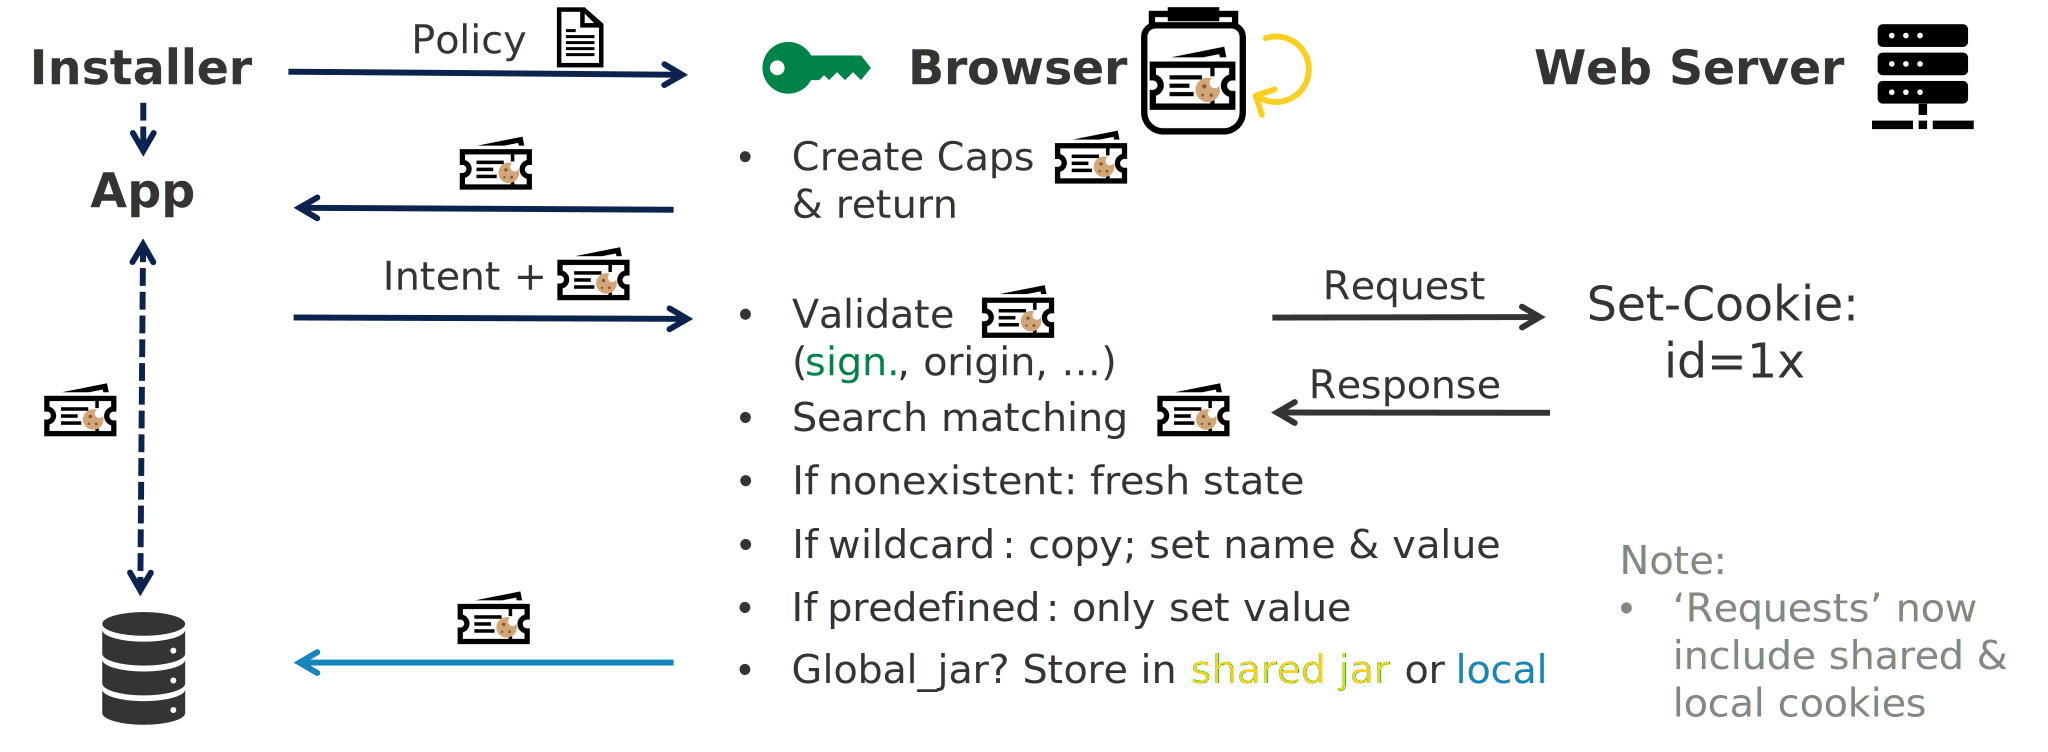
\includegraphics[width=0.9\textwidth]{ByeTrack_Flow.pdf}
  \caption{High-level overview of the Byetrack flow between installer, app, browser, and web servers.}
  \label{fig:byetrack_overview}
\end{figure}

To mitigate cross-app tracking caused by shared browser state, we propose a developer-defined policy mechanism, combined with cryptographically enforced capabilities, to control how cookies are managed and isolated on a per-app basis.

\section{The Policy}
To benefit from the scheme, the app developer defines a policy specifying which domains should share browser state and which should isolate it.
Optionally, the developer can also predefine specific cookie names expected from certain domains for more fine granular control.
This granular control goas beyong the simple trusted/untrusted domain distinction, allowing developers to specify exactly which cookies should be shared and which should be isolated, especially useful in scenarios where the developers wants to embed own domains that might host both first-party and third-party content.
If no policy is provided, the defense allows backwards compatibility by reverting to the default behavior of storing all cookies in the browser's shared jar.
This way, the developer can choose to not implement any policy and still have the app function as before, albeit without the privacy benefits of the proposed mechanism.

\section{The Capability Token Structure}
Each capability token defines the following fields:

\begin{itemize}
  \item \textbf{Cookie Name and Value:} Represent the actual cookie data to be stored and managed by the browser.
  \item \textbf{Signature:} Ensures the capability was issued by the browser and has not been tampered with.
  \item \textbf{Package Name:} Identifies the origin of the CT or TWA request, ensuring that only apps that were initially granted this token can make use it.
    This field is essential to prevent implicit delegation -- without it, a receiving app could exploit the capabilities granted to the sending app and potentially gain unauthorized access.
  \item \textbf{Domain:} Specifies the designated destination web server, ensuring only capabilities issued for the domain launched will be considered to define the isolation scope for cookies received from that server.
    Otherwise, a malicious library included in the app could exploit capabilities issued for trusted domains to mislead the browser into storing cookies from untrusted domains in the shared global jar.
  \item \textbf{App Version Number}: Indicates the version of the app to detect potential policy changes and ensure consistency between app and policy.
    In case of a version mismatch, the browser rejects these capabilities.
    Every time the app is updated, the installer resends the policy to the browser, which can then issue new capabilities that overwrite the previous ones.
  \item \textbf{Rights:} Define the scope of access granted to the app --, whether it may request the browser to read the cookie name or value, or even write a cookie value.
    This restriction is essential to prevent libraries from exploiting browser access to extract capability values, which could otherwise be used for tracking, for example HyTrack that could use the cookie name as the identifier instead of the name.
  \item \textbf{Global Jar Flag:} Determines whether the shared cookie jar or an app-specific cookie jar should be used, i.e. whether the cookie should be send back to the app to be stored in its isolated jar or kept in the browser's shared jar.
\end{itemize}

We distinguish between \textit{final} and \textit{wildcard} capabilities. Final capabilitiies are fully specified, containing fixed cookie names and values, while wildcard capabilities leave these fields unspecified, allowing the browser to fill them in dynamically when cookies are received from the web server -- thereby creating \textit{final} instances of capability token.
Therefore, the wildcard capabilities can be seen as templates for generating final capabilities on-the-fly, which fall into one of the following categories:

\begin{itemize}
  \item \textbf{Classic Wildcard Capabilities:} The classic wildcard capability leaves wildcard fields for both cookie name and value.
    This token can either exist to state that all cookies from a specific domain should be stored in the global cookie jar or in the app-specific jar, depending on the global jar flag.
    Consequently, this means one of such token is sufficient per domain to either allow or disallow sharing of all cookies from that domain.

  \item \textbf{Predefined Capabilities:} Allows the developer to specify particular cookies by name are expected from a specific domain.
    This provides fine-grained control over cookie scoping and allows developers to isolate their app from the browser's state when desired, while still enabling seamless web-app integration.

  \item \textbf{Ambient Capability} Instruct the browser to revert to default behavior by storing all received cookies in the global cookie jar and including them in subsequent requests to the corresponding web server.
    These have the global jar flag set by default and augment a wildcard capability with the domain name, cookie name, and corresponding value.

    \textit{Note: The Ambient capability provides no security guarantees and serves solely as a fallback mechanism for maintaining functionality when no explicit developer policy is provided.}
\end{itemize}

% Developer Policy Declaration
\section{Capability initialization flow}
During app installation, the installer extracts and transmits the policy to the browser.
Before creating any capability tokens based on the received policy, the browser validates and, if necessary, downgrades the policy to ensure minimal privilege.
This downgrade step prevents ambiguous or conflicting entries from resulting in overly permissive capability tokens.
The downgrade follows these rules:

\begin{itemize}
\item Predefined conflicts:
If a domain or cookie name appears under both predefined global and predefined private, the global entry is discarded and replaced by the private one.
This ensures that private capabilities (i.e., those restricted to the app’s private cookie jar) always take precedence over global capabilities.

\item Cookie-level conflicts:
If the same cookie name occurs in both global and private lists for the same domain, only the private entry is retained.
This prevents a single cookie from being accessible with two different privilege levels.

\item Wildcard conflicts:
If the same domain appears in both wildcard global and wildcard private, the domain is downgraded to private.
This ensures that domain-wide capabilities default to the least permissive (private) scope.

\item Independence of wildcard and predefined sections:
The predefined and wildcard sections are treated independently.
This means a global predefined rule (e.g., for a specific cookie) and a private wildcard rule (e.g., for all other cookies on the same domain) can coexist.
Likewise, a global wildcard and private predefined entry may both exist for the same domain.
These combinations are allowed because they describe complementary rather than conflicting access scopes.
\end{itemize}

The result of this downgrade process is a sanitized, conflict-free policy that preserves legitimate combinations of predefined and wildcard entries, while eliminating overlapping or inconsistent privilege assignments.
This ensures that capability tokens generated from the downgraded policy follow the principle of least privilege, minimizing the attack surface if an app misconfigures or intentionally inflates its declared policy.
The generation process itself is straightforward:
If the policy contains predefined entries, the browser generates corresponding predefined capability tokens for each specified domain and cookie name.
If the policy contains only a domain stating that all cookies from this domain should be stored in the global jar, the browser creates a classic wildcard capability for this domain with the global jar flag set accordingly, and vice versa for the private jar.
If no policy is provided, the browser creates an ambient capability with the global jar flag set, effectively reverting to the default behavior of storing all cookies in the shared jar.
Finally, each token is signed, ensuring its authenticity and integrity before being encrypted to ensure the tracking library cannot even read its contents to conduct tracking by leveraging cookie names or values.

After successful generation, the browser sends all created wildcard capability tokens to the app, which stores them in its private wildcard storage for future use.
The browser also lets the app know whether the app runs in ambient mode or not, i.e., whether a policy was provided by the developer or not.
This is important for the app to know whether the token it received was the ambient capability or another token, as they are encoded and encrypted and thus indistinguishable for the app.
Note: The app also stores the final capabilities separately in its private final storage, which are initially empty and may only be received upon requests to the web server.

Storing the wildcard and final tokens separately serves solely implementation convenience, as discussed in the implementation chapter \ref{chap:implementation}. % TODO keep this or remove?

When the app is updated, the installer resends the policy to the browser, which can then issue new capabilities that overwrite the previous ones.

% App-to-Browser Communication via Capabilities
\section{CT and TWA workflow with our capability mechanism}
When the app opens a URL via CT or TWA, the wilcard tokens (and up to this point empty final stokens) are attached to the respective intent used to start the activity.
After successful decryption of the received capability tokens, the browser parses and verifies their authenticity by validating the signature, the app package name, version number and the destinatin domain.
If any of these verifications fail, the browser discards the capability token and treats it as non-existent.
Otherwise, the valid wildcard capabilities are used to (1) manage cookies received from the web server and the valid final capabilities are used to (2) construct a cookie header.

Upon receiving cookies, the browser matches them against the capabilities it holds for the browsing context provided by the app.
The browser then processes each cookie with descending priority as follows:
\begin{enumerate}[label=\arabic*.]
  \item If the token is ambient, the browser directly stored the cookie in the shared cookie jar, like it would do without any capability mechanism in place.

  \item If a private predefined capability exists matching the name of the received cookie, the browser only fills in the matching cookie value in the capability and returns it to the app to store it in its isolated jar.
  \item If the browser holds a private wildcard capability, both the cookie name and value are filled in accordingly and the capability is returned to the app for storage in its isolated jar.
  \item If a global predefined capability exists matching the name of the received cookie, the browser stores the matching cookie in its shared jar.
  \item If a global wildcard capability exists, any cookie received from the webserver has permission to be stored in the browser's shared jar.
  \item If neither a predefined nor a wildcard capability exists, the browser discards the cookie and it is never stored.

\end{enumerate}

When sending requests to the web server, the browser utilizes the valid final (in-app) capabilities received from the app to construct a cookie header.
The browser merges the resulting cookie header with the cookie header created from the shared cookie jar by default and sends it to the web server.

The communication between browser and web server remains unchanged, i.e. the browser sends request and set-cookie headers as usual and the web server responds with a (customized) response and possibly new cookies.

\section{Additional Utility}
To enhance usability and developer experience, our mitigation framework includes additional utility that allow to get insights about the current final capabilities held by the app and thereby make use of the predefined capabilities.
For this, the app can query the browser to (1) get the names of the cookies encapsulated in the final capabilities, (2) retrieve the cookie values of final tokens and (3) write/update cookie values in final tokens.
The browser only grants these requests if the corresponding rights are granted in the capability token, that is read rights for (1) and (2) and write rights for (3).

\section{Benefits} 
Beyond eliminating cross-app tracking through HyTrack and its postulated goals, we identify the following additional benefits offered by our approach:
\begin{enumerate}[label=B\arabic*)]
  \item \textbf{Fine-Grained Control}: Developers can specify which cookies are shared and which are isolated, allowing for a more tailored approach to privacy.
  \item \textbf{No Browser State for Apps}: The browser is stateless with respect to app-specific capabilities, as these are retained and transmitted by the app with each intent invocation.
  \item \textbf{No Third-Party Code Changes}: The web server does not need to be aware of the capabilities or make any changes to its code, as the browser handles the capability management.
  \item \textbf{Backwards Compatibility}: In case the developer does not implement its own policy, it will default to allowing any domain using the shared browser state, consequently behaving like the state-of-the-art cookie management. 
\end{enumerate}

\section{Other Considerations}
Instead of the installer sending the app's policy to the browser, which then generates the capabilities accordingly and sending them to the apps, an alternative approach would be to let the installer directly generate the capabilities based on the policy and send them to the app.

This would free the browser from the resposibility of generating the capabilities and thus reduce its complexity to only enforcing them and would no longer require communication between installer and browser for each app.
For further deployment, this could be beneficial as the installer is part of the OS and thus does not require updates like the browser would, such as only require cooperating browsers to only implement the enforcemt.
However, this would require a decentralization of the token functionality and thus require the installer and browser to initially share a secret key, which increases the trusted computing base and thus the attack surface.
Therefore, we decided against this approach and chose the browser as the sole trusted component responsible for capability generation and enforcement for our proof-of-concept.

% TODO: What about bootstrapping 

% -----------------------------------------------------------------

% % Hypotheses    (ONLY NEEDED FOR PRPOSAL?)
% \section{Hypotheses}
% The evaluation is based on the following hypotheses:
% 
% \begin{enumerate}[label=H\arabic*)]
%   \item Passing capabilities with each intent enables the browser to validate and manage cookies securely and effectively. It also ensures the browser does not need to store app states.
%   \item The custom installer reliably transmits developer-defined policies to the browser.
%   \item The proposed mechanism is compatible with the original three goals of HyTrack as outlined in Section~\ref{chap:eval}.
%   \item The mechanism significantly mitigates cross-app tracking by isolating browser state based on trusted policy definitions.
%   \item The use of \textit{Ambient Capabilities} ensures backwards compatibility with existing systems.
%   \item In the case of invalid or missing capabilities, the browser by default discards the received Cookie, preventing fallback to shared state.
%   \item The proposed approach requires no modifications to existing third-party web server code.
% \end{enumerate}
% 
% % -----------------------------------------------------------------
% 
% %\todo[inline]{keep components section?}
% \section{Components}
% In summary, implementing the proposed solution requires a combination of new components and modifications to existing ones:
% \begin{itemize}
% \item \textbf{Manifest} and \textbf{config file} for the developers to define which origins should retain shared browser state.
%   \item A \textbf{custom installer} to extract and send the developer-defined policy to the browser upon app installation.
%   \item The \textbf{browser} to function as the Policy Enforcement Point.
%     For this, new functionality for validating the received policy, creating capabilities accordingly and validating them is necessary.
%     In addition, the browser needs to be capable of storing a secret key for signing capabilities and verifying the signature.
%     Of course, functionality for making decisions based on the capability's context is essential, i.e. where and how to store the capability.
%   \item The \textbf{app} must send capabilities as an additional parameter with each intent and store the capabilities returned by the browser for future use.
%     It must also support functionality to send specific capabilities to the browser.
%   \item \textbf{Capabilities} to serve as secure wrappers for cookie data, including the app ID, target domain, global jar flag, and associated access rights.
% \end{itemize}

